\section*{Project Description}

% \SECTION{A}
% Ref A = \ref{A},
% Ref B = \ref{B},
% Ref C = \ref{C}
% \SECTION{B}
% \SUBSECTION{C}

% \section{A}\label{A}
% Ref A = \ref{A},
% Ref B = \ref{B},
% Ref C = \ref{C}
% \section{B}\label{B}
% \subsection{C}\label{C}

\iflater\todo{Remember to not use any URLs in the project description!
  (They are encouraged in the references.)}\fi

Testing plays a vital role in modern software development processes,
contributing crucially to robustness and overall quality---as well as
to overall development costs.
%
It comes in many styles---unit testing, integration testing,
performance testing, stress testing, accessibility testing,
etc.---supported by many sorts of tools, with yet more advanced tools
and techniques continually being developed, studied, and applied.

One such technique, {\em property-based testing} (PBT), has been
enthusiastically taken up by the functional programming research
community, since its introduction in the QuickCheck
library~\cite{ClaessenHughes00} in Haskell, and is beginning to make
serious inroads beyond academia.
%
PBT is sometimes explained as ``formal specification without formal
verification''---a developer characterizes a the desired behavior of
some piece of code at a high level, in the form of executable {\em
  properties}, which are simply Boolean-valued functions; the code is
then validated against these properties by running it over and over
with a large number of automatically generated test cases.
%
PBT tools thus give programmers an efficient way of testing their
software's behavior with a comprehensiveness that is often not
possible with alternative tools.

PBT's combination of rich, high-level specification with easy, mostly
automatic validation has proved effective at identifying subtle
bugs in telecommunications software~\cite{arts2006testing}, replicated
file~\cite{hughes2014mysteries} and key-value
stores~\cite{Bornholt2021}, automotive software~\cite{arts2015testing}, and a range
of other real-world systems~\cite{hughes2016experiences}. With support
now available in all major programming languages, PBT has
begun to make significant inroads in the broader software
industry---for example, the developers of the Hypothesis library for
Python estimate that it has on the order of half a million
users~\cite{ZacPersonalCommunication}.

\newcommand{\participant}[1]{{P#1}}
% \newcommand{\participant}[1]{{\bf P#1}}

After all these successes, one might wonder if the research community has already
addressed all of the challenges that could limit PBT's adoption
in the broader software industry, but it
seems the answer is no.
In an ongoing need-finding study with users of OCaml's QuickCheck testing tool
at Jane Street Capital, we found
consistent enthusiasm for PBT---participants called it it
``obviously valuable'' [Participant \participant{1}],
built their own libraries for it when standard ones were not available in their
development context [\participant{8},
\participant{21}], and suggested that ``everyone'' at the company should use it
[\participant{20}]. But we also found
% \jsquote{28}{If you’re trying to build something that needs to be
%   reliable and work all the time, [PBT] is worth the
%   investment.\iflater\bcp{This is a paraphrase of what Dani said.  We
%     need to pull the actual quote. }\fi}
% \amh{This quote to me does not convey strong enthusiasm, but
% rather muted pragmatism :-). Maybe another quote would do
% the job better. Or maybe we can include that quote from the
% pilot study which stated that PBT was 1000x better
% than the alternatives.}
challenging new research questions based on developer concerns.
Specifically, the developers we have spoken with so far
%
(a) sometimes struggle
to identify all the situations where properties are readily accessible for
testing,
%
(b) they complain that it
can be difficult to write random generators for data structures
with complex invariants or to tune generator distributions to
adequately explore the space of interesting test cases,
%
(c) they find
it hard to understand whether their properties and generators are
effectively testing their software, and
%
(d) they are disappointed by
the paucity of educational and training materials for introducing
newcomers to PBT.\iflater\bcp{All that needs final tuning.}\fi

Solutions to these challenges will demand insights from both the
programming languages (PL) and
human-computer interaction (HCI) communities.  Chasins et
al.~\cite{chasins_pl_2021} argue that PL+HCI is a ``sweet spot'' that marries
``need-finding techniques [to] identify ...  programmers' current and future
pain points'' with tools that ``help [programmers] write safe and correct
programs.'' We wholeheartedly agree.

We propose a comprehensive, interdisciplinary research program that
will bring the combined power of PL and HCI approaches to bear,
accelerating PBT's transition into practice\iflater\bcp{do we need
  this?} and creating a blueprint for further research\fi.
% BCP: I really think this is not needed (readers will figure it out),
% and it weakens the rhetorical punch:
%   After an orientation to
%   PBT and discussion of our motivating study, we discuss the following lines of
%   work:
\iflater\hg{I think the Orientation section is too dense (and long) to make it clear
that the motivation is coming. If someone sees orientation, thinks "OK, I know
PBT so I'll skip this and come back if needed" they may skip to D1 and miss
motivation by accident}\bcp{Maybe we can somehow add a reference to the
Motivation discussion in the first bullet?  (I'm still not so worried
about this, though.))}\fi
\begin{itemize}[noitemsep]
  \item
  Our ongoing study (described in more detail below) is
  just the first step in our formative research.
  We will further explore the challenges PBT faces in
  industry by conducting three additional
  studies---two survey studies and one observation study of
  PBT users {\em in situ} (\sectionref{sec:foundation}).
  \item We will address challenges in property specification by developing a
  conceptual framework of high-impact PBT use cases, along with tools that
  enhance PBT in common use-cases like model-based testing and extend that set
  of use cases with the ability to write properties over logged output
  (\sectionref{sec:spec}).
  \item We will address challenges in test-case generation with new
  domain-specific languages for expressing generators that enable novel
  algorithms for PBT tasks like generation of precondition-satisfying values,
  test input mutation, and example-based generator tuning.
  (\sectionref{sec:gen}).
  \item We will address gaps in validation of testing effectiveness by providing
  users with powerful new ways of interacting with their generators and test
  suites that give them visibility into the bug-finding power of their tests
  (\sectionref{sec:val}).
  \item We will create comprehensive educational resources for training developers and
  university students in best practices for PBT (\sectionref{sec:ed}).
\end{itemize}
We conclude the proposal with a concrete outline of our work plan
(\sectionref{sec:plan-of-work}) and discussion of the broader impacts of the
proposed work (\sectionref{sec:broader-impacts})

\iflater\bcp{This needs a bit of focusing and toning down at some point.}\fi
The projects we undertake will be motivated by
foundational need-finding research in the software industry, including, but not
limited to, the aforementioned study with Jane Street. Some projects will have a
clear PL flavor, focusing on domain-specific languages and type-based tools that
will make PBT tools more powerful and flexible; but we will motivate and
evaluate them with techniques from HCI. Other projects will focus on the HCI elements
of PBT, building better interfaces and experiences for developers; yet their
implementation will draw from our wealth of PL knowledge. In this way, we craft
a holistic research agenda around PBT that is sure to be both well motivated and
well founded.

% Testing plays a central role in modern software development,
% contributing crucially both to the costs of software projects and to
% the quality of their results.
% %
% Testing comes in many styles---unit testing, integration testing,
% performance testing, stress testing, accessibility testing,
% etc.---supported by many sorts of tools, with yet more advanced tools
% and techniques continually being developed, discussed, and applied.

% One such technique, {\em property-based testing} (PBT), has enjoyed
% widespread popularity in the functional programming community since
% its introduction in the QuickCheck library~\cite{ClaessenHughes00} in
% Haskell.  PBT can be thought of as a kind of ``formal specification
% without formal verification.''  Programmers are invited to
% characterize the desired behaviors of their software systems or
% individual components at a high level, in the form of abstract models
% or algebraic laws; their code is then validated against these
% specifications by running it against a large number of automatically
% generated test cases.

% This combination of rich, high-level specifications with easy, mostly
% automatic validation has proved extremely effective at flushing out
% bugs in telecommunications software~\cite{arts2006testing}, replicated
% file~\cite{hughes2014mysteries} and key-value
% stores~\cite{Bornholt2021}, cars~\cite{arts2015testing}, and a range
% of other real-world systems~\cite{hughes2016experiences}.  With PBT
% tools now available in pretty much every major programming language,
% PBT has begun to make significant inroads in the broader software
% industry---for example, the developers of the Hypothesis library for
% Python estimate that it has on the order of half a million
% users~\cite{ZacPersonalCommunication}---creating large benefits in
% productivity and software quality for its users.\iflater\bcp{Can we
%   justify that?}\fi

% What would it take to make the benefits of PBT available to an even
% broader community of software developers?  Maybe not so much.

% In an ongoing study of users of OCaml's QuickCheck testing tool at
% Jane Street Capital, a Wall Street financial firm, we have heard
% strong enthusiasm tempered by a degree of frustration on a few fronts.
% These users generally appreciate PBT for its power and broad
% applicability, but (a) they sometimes struggle to identify
% situations where PBT will be valuable,
% (b) they complain that it
% is sometimes difficult to write random generators for data structures
% with complex invariants or to tune generator distributions tg
% adequately explore the space of interesting test cases, (c) they find
% it hard to understand whether their properties and generators are
% effectively testing their software, and (d) they are disappointed by
% the paucity of educational and training materials for introducing
% newcomers to PBT.  \iflater\bcp{All that needs final tuning.}\fi
% %
% Fortunately, we believe all these difficulties can be significantly
% improved with a modest amount of suitably focused research energy.  We
% propose to provide it.

% The remainder of this section introduces property-based testing and
% describes the findings of the Jane Street user study in more detail,
% to motivate and contextualize the work planned for this project.  The
% remaining sections describe several threads of planned work and their
% expected contributions.  Specifically, we aim to (1) further
% investigate the challenges PBT faces in industry through
% two\bcp{three?}  additional user studies (\sectionref{sec:spec});
% address the challenges we have observed in (2) property specification
% (\sectionref{sec:spec}), (3) test-case generation
% (\sectionref{sec:gen}), and (4) validation of testing effectiveness
% (\sectionref{sec:val}) by developing new, theoretically motivated and
% rigorously designed, tools; and (5) create comprehensive resources for
% educating developers and university students in best practices for PBT
% (\sectionref{sec:ed}).  \bcp{This is OK as a TOC, but as an
%   advertisement of planned contributions it is still pretty
%   lacking. We'll need to either add a separate contributions paragraph
%   someplace later or (better, I think) beef up this one.}
% \bcp{Need to mention broader impacts and work plan sections.}

\subsectionstar{Personnel}
%
\todo{One paragraph about what a great team we are, how the PI
  qualifications complement each other, and what kind of students we
  aim to support.  To make it fit smoothly here, concentrate on the
  interdisciplinary nature of the project.  Or maybe we should just
  add a bit about the team to the end of the PL+HCI paragraph above?}
% We have seen these trends firsthand: the PL research group at Penn has
% contributed to PBT research for years, pushing PBT to its limits as a
% tool for standard
% testing software~\cite{hughes2014mysteries, li_model-based_2021,
% goldstein2021dojudgeatest, goldstein2022parsing} and adapting it to new domains
% like theorem proving~\cite{paraskevopoulou_foundational_2015,
% lampropoulos_coverage_2019}.  The community has dedicated itself to improving
% the theory and applications of PBT, and recent work has continued to make great
% strides in areas like expressivity and testing effectiveness.


\sectionstar{Orientation: Property-Based Testing}
Before discussing our motivating study, we briefly explain what PBT is
and why it is important.

PBT is a form of random testing~\cite{hamlet1994random} where
users write executable functions, usually in the same language as
their System Under Test, which act as partial
specifications of a function under test. For example, a user might
write the following property of the \lstinline{insert}
function for an implementation of a binary search tree (BST):
\begin{lstlisting}
  prop_insertCorrect x t  =  (isBST t ==> isBST (insert x t))
\end{lstlisting}
This property takes only a single
line to express, yet it can be used to validate a limitless number of
input-output pairs. Concretely, it is
a simple function that takes two arguments and returns a
Boolean value: true if the property is satisfied, and false if it is
not. The function \texttt{prop\_insertCorrect} checks
that an insert operation on a binary search tree preserves the
binary ordering of the tree; it states
that, given an arbitrary tree \texttt{t} and an integer
\texttt{x} to insert into that tree, if the original tree
satisfies the
binary search tree invariant (``\texttt{isBST t}''), then it should remain
a BST following the insertion of \texttt{x} (``\texttt{isBST (insert x t)})''.

\iflater \bcp{I think this point will show up later:}There are a
myriad of different kinds of properties that one might use to specify
a system; a good source of examples is \citet{HowToSpecifyIt}.  \fi

Given a property like this one, the PBT tool chooses large number of inputs and
checks that the property evaluates to \lstinline{True} for each input; any input
that causes the property to fail is reported as a {\em counterexample}.  This
proposal is on property-based {\em random} testing~\cite{hamlet1994random}, in
which these inputs are chosen randomly.
\todo{There are other approaches, including} enumerative test-case generation~\cite[etc.]{DBLP:conf/haskell/RuncimanNL08, leancheck} and model
checking, but random generation remains the dominant approach in the PBT
space. Its surprising effectiveness is often attributed to the
``combinatorial'' nature of larger test cases: bugs can often be
exposed by test inputs with a specific combination of features,
independent of whatever other features may be present---for example,
by any sequence of API calls that includes calls to four particular
functions in a particular order, even if these calls happens to be
interleaved with other API calls.  This means that testing with one
big structure has the effect of testing with exponentially many
smaller sub-structures. Both practical experience and theoretical
arguments~\cite{goldstein2021dojudgeatest}\hg{?} suggest that this effect is quite
powerful---i.e., we can discover small counterexamples by generating
a few larger test inputs containing combinatorially many diverse
sub-structures rather than systematically enumerating test inputs
beginning with the smallest ones.

From the perspective of a user, applying PBT happens in a series of steps:
(1) Define one or more properties that should be true of the program under
  test.
(2) Design (or otherwise obtain) {\em random input generators} for the
  values that the properties take as input.
(3) Check the properties with generated inputs, using infrastructure
  provided by the PBT framework.
And (4) if counter-examples are found, make sense of them and determine the
  source of the bug.
Each of these steps presents opportunities to improve the user experience of
PBT, as we shall see below.
% How's that?
% ; when applicable, we will make it clear which of our projects targets which
% of these steps.\todo{Do that?}

\bcp{This is also the place to make our strongest argument for
  potential impact: Why is PBT so much better than standard unit and
  integration testing (at least sometimes)---e.g., its thoroughness,
  ability to discover weird edge cases, value as documentation, ease
  of application (in some common cases), ... what else?} \amh{+1}

\bcp{This is probably the place to mention a whole ton of related
  work, no?}

 \todo{Talk about fuzzers.}\hg{Probably, yeah. I have an
intro for it somewhere, we just need to hoist it}

\sectionstar{Motivation: A Formative Study of PBT in Industry \pagebudget{2}}\label{sec:motivation}
%
The concrete technical goals of this proposal are grounded in early
findings from an ongoing need-finding study asking {\em How can the
  research community make PBT more valuable for software developers?}
%
\iflater \todo{Sentence to justify why
we did the study}\bcp{If needed...}\fi
%
% \subsectionstar{Study Population}
%
To address this question, we conducted semistructured interviews with
stakeholders at Jane
Street Capital, including both
developers who have had exposure to PBT as
well as developers of PBT tools.
Questions focused on tasks that developers wish to
accomplish with PBT tools and developers' recollections of what it was like to
work with PBT tools to accomplish these tasks.

Interview
studies are common in early-stage need-finding research, due to their ability
to yield highly informative stories about people, the tasks they need to
accomplish, and the tools they use to accomplish them. The purpose of these
interviews is to identify a broad set of opportunities for improving PBT tools,
grounded in concrete, authentic, detailed stories from developers.

Jane Street is one of the world's largest
financial market-makers; its 1700 employees
include around 700 software developers.  A number of features make
it an attractive place for this study.  Most importantly, PBT is
already well established at Jane Street, so there is a large
population of people with well-informed opinions on its benefits and
challenges.  Also, Jane Street famously builds almost all of its
software in OCaml, a mostly functional programming language with
strong support for static typing and modularity and a well-engineered
PBT tool. This unified
ecosystem allows us to control for a number of potentially confounding
factors: all of the developers have access to the same tools,
libraries, language-level programming abstractions, house coding
rules, social conventions, etc.

\iflater\bcp{Not sure we need to say all this?}
Ideally, these interviews would have included both current
users
of PBT as well as non-users of PBT. In reality, it is difficult to recruit and
have meaningful conversations with non-users of a technology. Our strategy was
to recruit across as broad a spectrum of usage as could be reasonably recruited
at our partner institution, including both frequent users of PBT technologies,
as well as a handful of
developers who have had only limited, occasional exposure to PBT. Our survey
study (\sectionref{sec:survey}) aims to establish contact with a broader
sample of non-users of PBT to assess opportunities for making PBT tools more
valuable and discoverable for this group.
\fi

Of course, findings from a study at a single firm with a homogeneous
OCaml-based testing ecosystem may not generalize outside of this
ecosystem. Part of our proposed work is to carry out further user
studies targeting a broader and more diverse community
(\sectionref{sec:foundation}).  However, Jane Street itself is quite
diverse in the sorts of software it builds, including real-time
trading, quantitative algorithms, networked systems, and hardware
description code~\cite{signalsandthreads}, and our study participants
come with a wide variety of experiences and requirements.

Our interview instrument---the script that we used to loosely
structure the interviews---and our analysis process were developed and
tested through a prototype study with seven users of the Hypothesis
PBT toolkit, recruited over Twitter.  This analysis yielded a
conceptual framework of barriers to usage of PBT, which we published
recently at the SPLASH HATRA workshop, one of the key venues for
emerging work on human aspects of formal methods tools and type
systems~\cite{goldstein2022some}.

The study format was semi-structured interviews exploring developers'
experiences and impressions of PBT. At the time of writing, the full
complement of 30 interviews and a preliminary round of analysis have
been completed; full-scale analysis will begin in 2023.

\subsectionstar{Organizing Themes} The main theoretical output from
this qualitative study will be a collection of themes that summarize
and categorize our observations about the ways Jane Street developers
use PBT, what they need from it, and how the research community be
able to help.  While deep analysis of the interview transcripts has
not yet begun, several themes are already apparent in our real-time
notes, and these form the backbone of the present proposal.

\newcommand{\proptheme}[1]{{\color{nord-orange} \em #1}}
\newcommand{\gentheme}[1]{{\color{nord-green} \em #1}}
\newcommand{\evaltheme}[1]{{\color{nord-purple} \em #1}} One set of
themes revolves around the {\bf specifications} that developers test.
% and the kinds of programs in which they choose to test them.
Since
PBT is often described as a kind of lightweight formal method, one
might imagine that a central challenge would be coming up with the
right specifications. Indeed, a smaller pilot study of PBT users in
Python that we ran to prepare for the Jane Street
study~\cite{PilotHypothesisStudy}\iflater\bcp{Is this the first
  mention of the pilot study?  If not, move this citation earlier and
  no need for it here.}\fi{} concluded just that. But at Jane Street
we actually heard very little about difficulties coming up with
properties; rather, most participants described applying PBT in
\proptheme{High-Leverage Scenarios} where properties were already
available or quite easy to imagine. This suggests that an effective way
to approach education and documentation around PBT may be to focus on
``opportunistic'' applications of PBT as an easy on-ramp.
%
% But while focusing on easy applications of PBT may be helpful for education and
% adoption, it feels disappointing\bcp{blah} from a research perspective. Luckily,

Our interviews also identified several \proptheme{Opportunities for
  Better Leverage}---situations where PBT is not easy {\em yet}, but
could be with a little more research effort.\bcp{Quick
  examples?} Furthermore, participants spoke at length about one
particular kind of PBT they do often, commonly called
\proptheme{Model-Based Testing}. Model-based testing is not so much a
scenario in which to apply PBT as it is a technique for using it, but
the interviews have given us ideas for how to improve model-based
testing in a way that may make PBT easier in some situations.
\bcp{huh?}
\bcp{Maybe add a forward reference to \sectionref{sec:gen}?}

Another set of themes concerns the {\bf generation} of
random inputs for property-based testing. Many participants spoke
highly of the \gentheme{Derived Generators} that can be inferred from the type system.
These generators are already quite good, but they could be better: participants
discussed both small (e.g., API quirks) and large (e.g., derived generators
cannot enforce semantic preconditions) deficiencies. When derived generators
failed, participants fell back to standard \gentheme{Bespoke
  Generators}, which
are far more flexible but proportionally more time consuming to design
and work with. There is significant room for improvement here.\bcp{A
  bit of detail, and a forward reference?}

If a generated input is deemed to be a {\em counter-example} for a
property, highlighting a bug in the code, it needs to be easy to use that
input to determine the root cause of the bug. The interviews made clear that
\gentheme{Shrinking}, the process of finding the smallest possible input that
provokes a given bug, is a critical part of the PBT process.\bcp{Also
  that there are problems to solve there?  (Otherwise, why are we
  mentioning it?)}

The final category of themes concerns the {\bf evaluation} of testing
effectiveness. In
general, with any sort of
testing, it can be difficult to know when ``enough is enough.'' In
standard unit testing, for example, developers may worry that test number
$n + 1$ will be the one that catches a bug; PBT does make it possible to to
automatically generate that one extra test, but one still has to decide when to
stop. This tension leads to a variety of approaches to
\evaltheme{Budgeting Time for PBT}: most of our interviewees run PBT
testing just for a few seconds per property, expecting
that the bulk of the necessary testing is done in hundreds or up to around a
thousand examples, but some run PBT for much longer. Interestingly, the opposite
is true about a close cousin of PBT, fuzz testing. Participants who used both
PBT and fuzzing tools ran the fuzzers for far longer (some for up to a CPU-year!).

It would be easier for developers to make informed decisions about
time budgets for testing if
they had better access to feedback about how well their testing is doing.
Indeed, \evaltheme{Evaluation of Effectiveness} turned out to be a common theme of our
conversations. There are many forms such feedback could take, from
code coverage to input space coverage measurements and even strategies like {\em mutation
testing}~\cite{papadakis_mutation_2018}; we hope\bcp{plan?} to explore the user experience
around many of these avenues.

\todo{Probably add quotes and stuff here to make this more
  interesting}\bcp{Maybe.  But we don't have space for too many.  (I
  guess if we don't format them in their own fboxes, we can fit more
  of them!)}

\iflater
\bcp{I think this can be cut?}What remains for this project is another
approximately 2 months of Ph.D.  student work, including conducting
the remaining interviews, performing in-depth qualitative analysis of
the data following a thematic analysis approach~\cite[Chapter
5]{blandford2016qualitative}, and preparing a manuscript for
submission to OOPSLA.
\fi

\iflater
\amh{Let's foreshadow other findings that
we will publish that are outside of the scope of this proposal, but which might
be motivating to other researchers, including: developers could benefit from
additional automated support for deriving generators from types, effectiveness
budget (i.e., deciding how much time to spend on running PBT tests versus fuzz
tests), integration with unit testing frameworks, and exploring the use of
properties as a source of documentation.}
\bcp{Not sure where is the right place for this discussion (or if
  there will be space)...}
\fi

% \todo{Debugging doesn't really fit here...}


\SECTION{Foundation: Understanding Needs and Opportunities \pagebudget{1}}\label{sec:foundation}

% \amh{This section is around double its page budget. One reason is that I am
% probably being too heavy-handed in trying to justify the methodological choices.
% Help me figure out what to prune!}\bcp{Did some pruning! :-)}

The final results from the in-progress user study should paint a clear
picture of the benefits and challenges of PBT in the specific context
of Jane Street and other organizations with similar characteristics.  But to
fully understand the potential impact of PBT across the software
industry---and the factors that may limit its adoption---we need to
cast a wider net.
%
In this section, we describe three planned studies, drawing on mixed
methods in the service of producing a comprehensive and actionable
agenda for future research, in this research project and beyond---two
written surveys, one to assess the generality of these needs and obstacles
and one to identify potential for adoption of PBT tools
(\sectionref{sec:survey}), and an observation study to understand
particular tasks involved in PBT to guide the design of new algorithms
and interactive tools (\sectionref{sec:observations}).

\iflater\bcp{Somewhere, we need to mention the letter of support from
  JS.  I guess it belongs in the section where we describe potential
  further collaborations with them.}\fi

\SUBSECTION{Proposed Work: Surveys to Generalize Findings}
\label{sec:survey}

Our ongoing Jane Street study has already revealed a number of
opportunities to improve tools for property-based testing. To identify
others, and to better understand which of these opportunities are most
important for the research community to explore, we will conduct two
surveys, each with a broad sample of developers. These surveys aim to
(1) determine which obstacles observed in the interview study
represent widely experienced pain points with PBT tools and
(2) characterize the potential benefits of better tools to the
software industry as a whole.

\emph{Validation survey}. Our interview study has revealed
a number of issues with existing PBT tools, but it is not clear
how broadly these issues are experienced by developers, or
their relative severity. To find out, we will conduct a survey
asking developers which of the issues we have identified are
ones they have experienced, and the severity of those issues
in their experience. Respondents will also be asked to report on
other issues that have arised in their use of PBT tools.
To provide
clear usage scenarios to guide future work, respondents will
be asked to write brief anecdotes elaborating on the
most severe issues they encountered.

Respondents will
be recruited broadly, from three sources. First, we will recruit
users of Hypothesis, a widely-used Python-based PBT
framework
% \footnote{In personal communications, one of the
% maintainers of Hypothesis estimates that Hypothesis has
% approximately 500k current users. \amh{I am not sure if we
% should include this. It sounds too big to be true to
% me.}}
% BCP: Already mentioned at the top
(see the attached letter of support).
Second, we will distribute the survey at Jane Street, hoping to reach
a broader set of developers than we were able to interview.
And third, we will recruit users from social media by posting
survey announcements from the PIs' Twitter and Mastadon
accounts, tagging the functional programming and testing
communities. \amh{Do we have any connections that would give
us access to functional programming or testing-related
software development conferences?}\bcp{Sure.  What would we do with
them?}

\emph{Impact survey}. Is PBT the sort of
technology that could one day be used by every developer? To get a
sense of this, we survey ``proximal'' users of PBT---that is,
developers who do not use PBT currently, but who experience
use cases where PBT methods would be particularly useful,
once designed to fit their tasks and workflows. Particular
attention will be given to those whose work requires the
writing of validation code and public APIs with some
definition of types. We will recruit a broad sample of
participants across development contexts (professional, open
source, educational) by working with our industry contacts
and by recruiting over social media. \amh{I am not sure this
survey feels quite right. It feels really hard to conduct in
a way that we get a convincing answer to our question of
``who would use PBT if the tools were sufficiently
well-designed?''}\bcp{Indeed---feels weaker than the other.}

\SUBSECTION{Proposed Work: Observations of PBT in Practice}
\label{sec:observations}

Anecdotes related in interviews do not generally, in and of
themselves, provide enough information to inform the design of
effective tools---they beg questions like: (1) How much time
are participants willing to devote to
a task like creating a generator or debugging a counterexample when in the
middle of a programming task? (2) How much space is available on a developer's
screen (amidst other tools like code editors and terminals) for
interacting with new
tools? (3) What are developers' current strategies for solving the
problems they describe
(for example, what representations of generated data currently seem most helpful
for programmers trying to under the distributions of data generated by a
generator)?.  As a basis for designing tools with a substantial novel interface
component\bcp{add forward reference...}, we will observe developers
undertaking the respective PBT tasks we
aim to support, on the order of a small handful of developers (i.e., 2--10
observation sessions). These observation sessions will allow us to evolve
singular anecdotes from the interviews into a more comprehensive picture of
what kinds of designs will be viable for helping programmers.

% \bcp{Again, we need to explain the expected contributions---what end
%   does ``characterizing obstacles'' serve.}

\smallskip

Together, the studies described in this section provide a firm
foundation for the rest of the proposed
activities, in the form of a validated and prioritized set of developer
needs for PBT tools and a detailed set of requirements for how tools should be
(re)designed to best satisfy the most important of those needs.
\bcp{Does that mean that the rest of the activities can only be
  started once these studies are complete??  (More generally, let's
  work on the Work Plan!)}

\SECTION{Specification: Widening the On-Ramp \pagebudget{2}}\label{sec:spec}

\bcp{...and this one should open with a continuation of the transition
that suggests how these particular projects are motivated and informed
by all the studies.}

\SUBSECTION{Proposed Work: When to Specify It!}
PBT is often described as a kind of lightweight formal method, and one
might therefore imagine that a central challenge of using PBT would be
coming up with the
right specifications. Indeed, our pilot study concluded just that. But at
Jane Street we actually heard very little about the challenge of coming up with
properties; instead, most participants described applying PBT in scenarios when
properties were already available or quite easy to imagine. This suggests that,
while PBT educators should certainly spend some time teaching developers how to
write specifications for arbitrary programs, they should spend even more energy
helping developers quickly recognize  situations where PBT is a particularly
natural fit because properties are obvious!

With this in mind, we plan to write a paper
(with an accompanying talk)
entitled {\em When to Specify It!} in homage to
John Hughes's {\em How to Specify It!}~\cite{HowToSpecifyIt}, a lovely
tutorial on the many different kinds of properties that one can write
for a given piece
of code. Clearly it is important to ask {\em How}, but our developer interviews
suggest that it may be even more important to have a clear sense of {\em When}
to use PBT. Our paper on {\em When to Specify It!} will combine examples from developer
interviews with ones from our our years of experience studying and applying PBT
into the definitive guide for the most impactful opportunities to apply PBT.
\iflater\hg{Do we need more here? I can give examples...}
\bcp{If they haven't already come up earlier, then yes, let's list
  some here!}
\fi
% \begin{itemize}
% \item Code that is already (semi-)formally specified.
% \item Functions that round trip.
% \item Pure data structures.
% \item Modules with invariants.
% \item Related versions of the same code.
% \item Programs that may fail catastrophically.
% \item Stateful APIs with well-understood contracts.
% \end{itemize}

\SUBSECTION{Proposed Work: Properties Over Output Logs}
One common problem raised by Jane Street developers (and even more loudly
in our earlier pilot study~\cite{goldstein2022some}) was
that code may sometimes not be abstracted
in a way that is amenable to PBT. Indeed, any kind of
testing of software units---using PBT techniques or otherwise---requires
``units'' to test!  But PBT is
especially sensitive to things like poorly encapsulated global state, which may
impact the repeatability of testing, and leaky or confusing
abstraction boundaries, which make it difficult to cleanly state
properties or specifications.  Fuzzing tools get around these issues by
testing code ``from the outside''---they do not care about internal
abstractions, only external interfaces---but this usually comes at the
expense of expressive properties.  \bcp{``but this usually comes at the
expense of expressive properties''---spell out what this means and why
it is so.}

We hypothesize a solution that enables better PBT,
especially in messy programs that do not have clean abstraction boundaries,
without giving
up expressiveness: inject logging calls into the code under test, and write
properties over the logs that the code produces. For example, if the developer
knows about some invariant on a variable \lstinline{x}, they can log out the
value of \lstinline{x} every time it is set, and then check that the logged
values satisfy the invariant. We plan to use meta-programming to automate this
process, so a user need only mark the variable to log its updates. Another
useful property over logs concerns
invariants that applies over time (e.g., the value of \lstinline{x} should
never decrease).
This would be difficult to do with debug assertions, since state would need to
be kept for arbitrary amounts of time between variable updates; setting up such
state may itself require some error-prone restructuring of the code, especially
if the debug state should be compiled away in release builds.

Concretely, we propose a framework for inserting lightweight test-logging and a
language for writing properties over those logs. The logging itself is a matter
of engineering, but the language for properties is an exciting opportunity to
apply powerful logical ideas. Specifically, the properties over logged outputs
should be written in a temporal logic like {\em linear temporal logic} (LTL) so
they can make complex assertions about the way past and future values interact.
The Quickstrom testing framework~\cite{oconnor_quickstrom_2022} has already shown that
LTL properties are possible (it uses LTL to write properties about graphical
user interfaces), and we will adapt those results to be useful for a much
broader set of programs.

\SUBSECTION{Proposed Work: Automating Model-Based PBT}
Our studies have shown that a common pattern of PBT, especially for stateful
APIs, is to implement a {\em model implementation} of the system under test, and
then check that the two versions of the code agree on a series of API calls.
This is a well documented approach to PBT~\cite{hughes_experiences_2016}, but it
is not always supported as well as it could be by existing tooling. For example,
developers at Jane Street cited setting up essentially the same basic
model-based PBT harness for at least three different projects; implementing each
of those harnesses took significant developer time and slowed down the testing
process.

We propose new, type-based automation for model-based testing of ML-style
modules. This automation will take a model signature, for example
\begin{lstlisting}[language=Caml]
  module Map : sig
    type ('k, 'v) t
    val get : ('k, 'v) t -> 'k -> 'v option
    val put : ('k, 'v) t -> 'k -> 'v -> ('k, 'v) t
  end
\end{lstlisting}
and generate a series of calls like
\begin{lstlisting}[language=Caml]
  let m = put m 1 2; get m 1; let m = put m 1 3; m get 1
\end{lstlisting}
that manipulate the data structure and query its contents. When testing two
different implementations of \lstinline{Map}, the developer can verify that the
two implementations produce the same results for each of the operations in the
sequence. The automated tooling could also insert checks for internal
invariants, ensure that one operation executes at least as quickly as another,
and insert other checks that are simple to specify but tedious to implement
manually.

Our choice to focus on ML-style modules is motivated from two directions. One is
practical: our relationship with Jane Street makes it easy to evaluate tools
that are compatible with OCaml, the language that almost all of their developers
are the most comfortable with. Working within the OCaml ecosystem will mean that
we can quickly find technical or usability issues with the tools we build. The
other reason, though, is technical interest. ML modules are extremely
expressive and fairly complicated. This gives us a number of complex problems to
solve: for example, \todo{Maybe have Joe look at this section. He really likes
this project}

\bcp{This all needs to sound more like research (as opposed to
  ``building a little tool for JS'')...  The unwritten bits should
  help. :-)}

\SUBSECTION{Proposed Work: Interactive Property Specification}

\bcp{General comment for this section: It all seems good, but it is a bit vague
and high level---I feel like technical readers will want a bit more meat.  Could
we spice it up with a concrete example?  (Indeed, should we be thinking about a
running example for the whole proposal?)} \amh{Agreed, I think a concrete
example would be \emph{great} here. Maybe there is an example we can bring in
from the QuickSpec paper~\cite{claessen2010quickspec}}

As our pilot interview study has suggested, developers sometimes have
difficulty imagining which properties to test, even when they know that their
software would benefit from property-based testing. One area we are interested
in exploring is how programmers can work with their PBT tools to decide on a set
of significant properties to test.  Prior research demonstrates that automated
tools can extract specifications of a program's
behavior\cite{ammons2002mining,le2018deep,claessen2010quickspec}. We are
interested in the non-trivial research problem of integrating such techniques
into usable developer tools. We see the research as addressing several
challenges:

\textit{Generated properties should be \underline{important}}. Any non-trivial
program can be characterized by an overwhelmingly large number of properties,
many of which describe only incidental aspects of the program's behavior that do
not need to be tested. How can tools produce those properties that developers
would want to have tested? We believe that this is a problem that can be best
solved with a mixed-initiative approach~\cite{allen1999mixed}, where properties
are determined by judiciously incorporating both developer input and automated
techniques.

Developer could guide a specification mining tool to extracting relevant
properties through input mechanisms such as (1) identifying regions of code that
are likely to lead to an adverse behavior such as an exception or a logical
error; (2) providing unit test cases that test a special case of a generalized
property; and (3) indicating aspects of interest on input and output data during
exploration in a debugging REPL.

\textit{Generated properties should be \underline{readable}}. While prior research\bcp{which?}
has shown promise for automatically generating specifications of program
behavior, we expect that users of PBT systems would benefit from having
properties generated in the language of their property-based testing tools.
Furthermore, there are some variants about systems that may be so complex that
they require significant comprehension time for users (i.e., those involving a
large number of clauses). In such cases, a tool may way to generate simpler
variants of properties first, and allow developers to refine them on their own.

\textit{Tools should help developers \underline{revise} properties}. If a generated
property is too relaxed, the tool should request that developer provides a
counterexample that should trigger a failure, and then regenerate the property.
If a generated property is too strict, a tool should allow a programmer to mark
a counterexample that was generated by the PBT tool as spurious, i.e., not
indicating an actual failure of the program. In each of these cases, the
property generator may have generate multiple properties for a developer to
review, each of which may satisfy the refinements that a developer has provided.

\textit{Plan of work}: We will iteratively design and develop developer tools as
an extension to the VSCode editor, a popular development environment for
Haskell. In our first iterations, candidate properties will be generated using
QuickSpec~\cite{claessen2010quickspec}. The interactions described above will be
designed and tested first for simple programs, and then on successively more
complex programs from our benchmark set. PI Head has extensive experience
designing and developing developer tools involving program
analysis~\cite{head2018interactive,head2019managing} and program
synthesis~\cite{head2017writing} components, and extending the VSCode
environment~\cite{head2020composing}.  \bcp{Maybe consider focusing on OCaml
tools, rather than Haskell, since this is where there might be synergy with Jane
Street?  Or do both?} \amh{This is a great idea. Does anyone know of any
specification generators for OCaml?}\bcp{No, but there is a ton of
follow-on work after QuickSpec (and related work before and
after)---we should make sure to cite it coherently.}

\SECTION{Generation: Better Tools for Random Inputs \pagebudget{3}}\label{sec:gen}
\hg{Half page over at the moment}\bcp{Made it a bit worse by moving
  the discussion of random vs. enumerative here... :-)}\bcp{And, just
  in terms of balance, spending 1.5 pages on context at this point
  feels excessive, unless we can really justify it in the narrative.}

One of the most important---and difficult---tasks in the PBT process is
designing and implementing the random data generators that are used check that
each property holds. Indeed, the developers we interviewed consistently
cited designing generators one of the hardest parts of the PBT process, and many
developers asked for better tools for constructing generators that accomplish
their testing goals. In this section, we describe a series of projects
to develop new and better ways to express random data generators.

\subsectionstar{Context: Why is Random Generation Hard?}%
Before presenting our proposed work to improve the state of random data
generators, we must first discuss the major difficulties with random generation
for PBT and the existing work that aims to address those difficulties.
\todo{Link all of this to the intro}

% \todo{Talk about enumeration}

{\em Preconditions.}
Many properties that developers want to test have {\em preconditions}
(equivalently {\em validity conditions} or {\em input constraints}) that
restrict the set of inputs that should be used for testing. This comes up often
when testing data structures with invariants that must hold in order to apply
the operations under test. Testing such properties can be problematic, because
many preconditions are difficult to satisfy randomly; if the developer is not
careful they may waste considerable time generating and discarding invalid inputs.

{\em Coverage of Realistic Inputs.}
Even among valid inputs, not all are equally realistic. Often generated inputs
feel fabricated, since they are not constructed with prior knowledge of the
kinds of inputs that the program is likely to see.

{\em Distributional Concerns.}
And {\em even} with validity and realism accounted for, there are other ways for
generators to under-perform. In particular, the spaces of inputs that generators
target is often very large, and the best generators explore as much of the space
as possible, as quickly as possible. This often (but not always) leads users to manually tune
the weights on generators' choices to ensure that the generator does not spend
too much time in one part of the space or another.

\todo{Make sure we tailor the explanations above to the problems we actually
solve, and then make it clear when we've solved one of the problems.}

The literature addresses these concerns to various degrees, and existing tools
fall on a spectrum from automatic to manual. The automatic approaches use
proxies for validity and general ``interestingness'' of inputs: some optimize
readily available metrics like code coverage~\cite{afl-readme}, others ask users
to provide metrics~\cite{loscher2017targetedpbt}, and naturally some use
machine learning to infer proxies for validity~\cite{godefroid2017learn,
DBLP:conf/icse/ReddyLPS20}. Slightly more manual approaches are based on
declarative representations of validity conditions: for preconditions that are
primarily structural, {\em grammar-based fuzzing} provides a compelling
solution~\cite{godefroid2008grammar, holler2012fuzzing, veggalam2016ifuzzer,
wang2019superion, srivastava2021gramatron}, and for more complex, semantic
preconditions, some have proposed using SMT-solvers~\cite{dewey2017automated, LuckPOPL, steinhofel2022input} to
automatically seek out valid inputs. This semi-automatic category also includes
tools for {\em example-based tuning}, a process that improves realism of inputs
by mimicking user-provided examples~\cite{soremekun2020inputs}.

The most manual, but also the most flexible, solutions use hand-written
generators, written in a convenient domain-specific language...

\subsectionstar{Context: Monadic Generators}
When writing generators manually, it helps to have a clean domain-specific
language (DSL) for writing them down. In the Haskell language, where PBT was
first popularized, many such DSLs are implemented using {\em
monads\/}~\cite{moggi1991notions}, an elegant design pattern for
expressing effectful (in this case, random and stateful) computations
in a pure, stateless underlying
language. While monadic DSLs are not actually necessary to express generators in
non-pure languages, some libraries (e.g., in OCaml) still use monadic
abstractions to build their generator DSLs.

Monadic generators implement random data producers of arbitrary complexity
(e.g., it is possible to write a monadic generator for Haskell
programs~\cite{palka_testing_2011}), so they are often more expressive than
other representations like grammar-based generators.  Yet monadic generators are
syntactically constrained in a way that isolates the probabilistic code and
prevents usage errors (like passing the wrong random seed around). As we will
see, the constrained nature of monadic generators also makes them the perfect
candidates for sophisticated manipulations and interesting generalizations.

\SUBSECTION{Prior Work: Free Generators}
In order to improve monadic generation along the dimensions listed
above, it helps to re-frame generators as {\em parsers of randomness}. A generator
operates by making a series of random choices, but we can equivalently think of
it as being provided some random sequence of choices and then simply following
those choices to produce a value. This perspective has been used in a few
implementations of PBT
systems~\cite{maciver2019hypothesis, dolan2017testing}; we made it
formal in our paper, {\em Parsing Randomness}~\cite{goldstein2022parsing}.

The paper introduces {\em free generators}, which generalize the standard
monadic generator abstraction, demonstrate a formal link between parsing and
random generation, and enable new algorithms for generation that improve
generation modulo validity constraints. Free generators are written the same
way as standard monadic generators, but they are more like generator ``plans''
or syntax trees.%
\footnote{Free generators are implemented using {\em freer
monads}~\cite{kiselyov2015freer}, which have been used to great effect in recent
years to capture the structure of effectful computations
(cf.~ITrees~\cite{old:xia2019interaction}). Freer monads represent
monadic computations syntactically by reifying the monad operations
(\lstinline{return} and \lstinline{>>=}) as data constructors. Critically, this
is all implemented within the language (no macros or AST
manipulation). See \cite{goldstein2022parsing} for more details on the
free generator representation.}
This means that a single free generator can be be {\em interpreted} in multiple
different ways. In {\em Parsing Randomness} we prove that any free generator can
be interpreted either as a standard monadic generator or as a source of
random choice strings with a parser over those strings; this formalizes the
relationship between generators and parsers. Furthermore, since free generators
are uninterpreted syntax trees, they can be manipulated programmatically. Free
generators admit a version of a Brzozowski
derivative~\cite{brzozowski1964derivatives} that can be used incrementalize
generation. We show that free generator derivatives enable an algorithm called
{\em Choice Gradient Sampling}, which uses repeated derivatives to guide a
generator to inputs that are more likely to be valid with respect to a given
precondition. This work is an important step towards better automation for
generators with complex preconditions.

\SUBSECTION{Ongoing Work: Reflective Generators}
Continuing on from the free generator work, we have begun to look at even more
powerful generalizations of the standard monadic approach to random generation.
One such project, which is already well underway, concerns monadic generators
that can be run {\em backward}.

If a generator parses a sequence of choices into a value, then running the
generator backward should take a value and produce a sequence of choices that
would produce that value. With this in mind, we present {\em reflective
generators}, an extension of monadic generators that can be run backward to
``reflect'' on the choices that they made when producing an input. The machinery
that makes reflective generators work is quite complex,%
\footnote{Reflective generators are both monads and {\em partial profunctors},
and implement bidirectional programming in the style of Xia et
al.~\cite{xia2019composing}. This approach to bidirectional programming is
related to lenses~\cite{foster2009bidirectional}, but it hides much of the
complexity of bidirectional program composition in the bind operation of the
monad. The result is an elegant programming experience where both directions of
the computation can be written at once in a type-safe way.}
but, like free generators, their syntax is still quite close to that of normal
monadic generators.

Reflective generators are useful for more than just generation; we currently
have two working examples of useful applications.

{\em Validity-Preserving Mutation.} Many automated testing algorithms
(especially fuzzing algorithms~\cite{afl-readme}) {\em mutate} values to explore
the behavior of the program in a space ``around'' those values. This can be
difficult in PBT scenarios, where values are subject to complex validity
constraints, since the mutation often produces invalid values. Reflective
generators can help: we can (1) reflect on the choices that lead to a particular
value, (2) mutate those choices, and (3) re-run the generator with the new
choices {\em while correcting any choices that
would lead to an invalid value.} Figure~\ref{fig:mutation} shows the way this
algorithm is able to mutate a binary search tree, while maintaining validity,
with no BST-specific code written other than the reflective generator.

\begin{figure}[h]
  \centering
  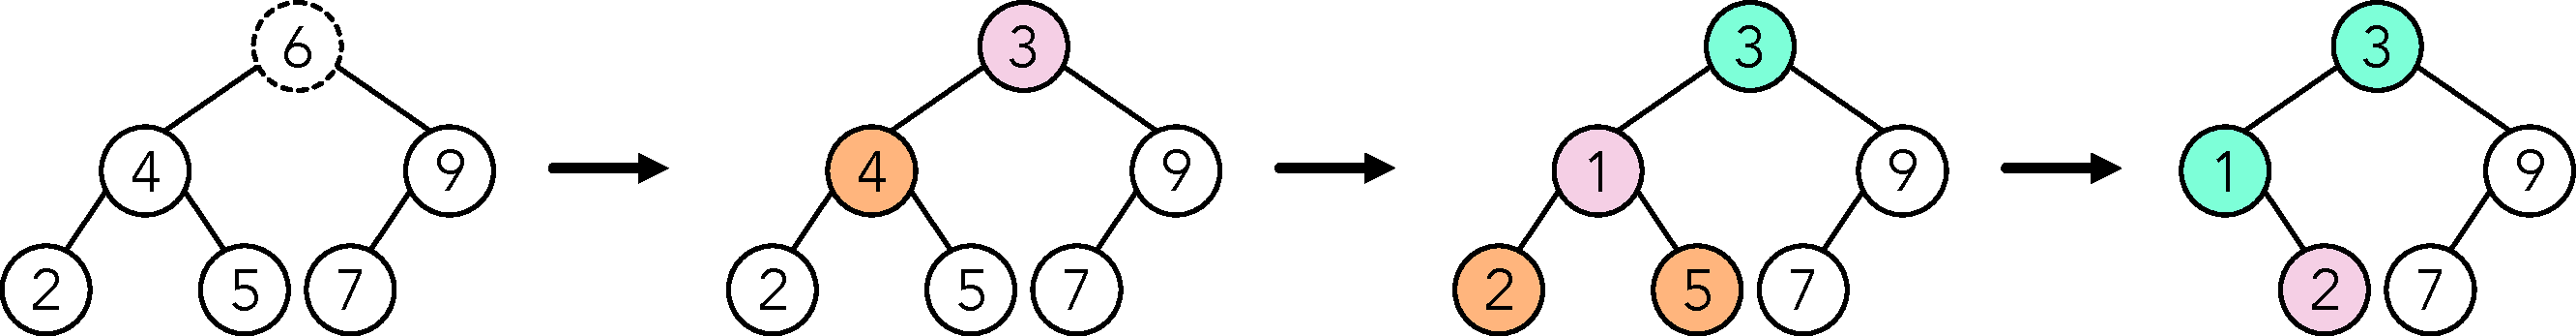
\includegraphics[width=.6\textwidth]{assets/mutate-diagram.pdf}
  \caption{Validity-preserving mutation of a binary search tree, maintaining the
  BST invariant.}\label{fig:mutation}
\end{figure}

{\em Example-Based Tuning.} Earlier we pointed out that good generators
produce ``realistic'' inputs; one way to ensure this is to tune the generator so
it produces values that are similar to some user-supplied values deemed
realistic. Existing tools make good use of this example-based approach to
tuning~\cite{soremekun2020inputs}, but they do not work with generators as
powerful as monadic generators. We implement a similar algorithm using
reflective generators: we can (1) again, reflect on the choices that lead to a
set of realistic values, and (2) run the generator with {\em new choice weights}
informed by the choices that we saw.

Both of these applications have the potential to significantly improve testing
effectiveness---example-based tuning helps users generate more realistic inputs,
adn validity-preserving mutation enables more automated approaches to improving
generator distributions---and we get {\em both} by upgrading our existing
generators to reflective ones. Additionally, we are confident that there are
more use cases for reflective generators, which we discuss more in the following
sections.

\SUBSECTION{Proposed Work: Bringing Fuzzing into Focus}
{\em Fuzzers} like AFL~\cite{afl-readme} use principles that are similar to the
ones behind PBT: they leverage randomized testing to quickly exercise as
many program behaviors as possible.  One might then expect that the fuzzing and
PBT share a significant amount of literature, but in reality they do not. Often
the communities seem to ``talk past'' one another.

We propose that the main thing separating the PBT and fuzzing communities is
simply a difference of {\em focus}. The fuzzing literature mostly talks about
fast and automatic ways to find critical (security) vulnerabilities in
programs---usually manifesting in the form of crash failures.  In contrast, PBT
researchers want effective ways to test semi-formal logical specifications of
their programs. Both areas of focus are important: fuzzing captures the ``80\%''
of cases catching high-profile bugs with minimal programmer effort, and PBT
gives a level of thoroughness that fuzzing does not claim to match. But there is
something unsatisfying when things are laid out this way. In particular, while
fuzzing and PBT focus on different testing problems, they face many of the same
technological hurdles. Both PBT and fuzzing need fast and effective ways to
generate random inputs that are valid for the systems that they are testing, and
neither community has truly settled on the ``right'' way to get there.

There is certainly some work that attempts to bridge the gap between PBT and
fuzzing. For example, FuzzChick library in Coq~\cite{OLDlampropoulos19fuzzchick}
uses code coverage as guidance for PBT and the HypoFuzz library uses a
similar approach in Python~\cite{hatfield-dodds_hypofuzz_nodate}. These projects
are demonstrably powerful, but neither benefits from the years of expertise
poured into actual fuzzers; Crowbar does~\cite{dolan2017testing}. Crowbar uses
AFL~\cite{afl-readme}, one of the most well-established
fuzzers, to generate random bit-strings that are later parsed into program
inputs.  (We plan to use AFL++~\cite{fioraldi_afl_2020},
which has supplanted the original AFL project.)  \bcp{Maybe this is a
  good place to mention Target, Learn\&Fuzz, Grammar-based fuzzing,
  etc.  Some paragraphs from Harry's thesis are in comments here.}

% A different approach that is {\em almost} entirely automatic is {\sc
% Target}~\cite{loscher2017targetedpbt}; it uses search strategies like hill
% climbing and simulated annealing to guide generation to more useful inputs.
% \citeauthor{loscher2017targetedpbt}'s approach works well when the notion of
% validity is in some way continuous (i.e., an input is not simply invalid, it is
% $X\%$ valid), but this is often not the case.

% Some approaches use machine learning to automatically generate valid inputs.
% {\sc Learn\&Fuzz}~\cite{godefroid2017learn} generates valid data using a
% recurrent neural network.  This solution seems to work best when a large corpus
% of inputs is already available and the validity condition is more structural
% than semantic. In the same vein, {\sc RLCheck}~\cite{DBLP:conf/icse/ReddyLPS20}
% uses reinforcement learning to guide a generator to valid inputs.

% For preconditions that are primarily structural, {\em grammar-based fuzzing}
% provides a compelling (if slightly more manual) solution. In {\em
% Grammar-based whitebox fuzzing}~\cite{godefroid2008grammar} a context-free
% grammar (CFG) is used to constrain the fuzzer's output. Over the years, many
% versions of this paradigm have been developed, including ones that use
% pre-written fragments of the input language to give the mutator interesting
% things to work with~\cite{holler2012fuzzing} and ones that use genetic
% programming to find more interesting inputs~\cite{veggalam2016ifuzzer}. The
% newest grammar-based fuzzing approaches use the grammar to do more structured
% mutation of values~\cite{wang2019superion,srivastava2021gramatron}. These ideas have also been integrated
% into PBT in the FuzzChick library~\cite{DBLP:journals/pacmpl/Lampropoulos0P19}.

% Moving into the range of ``mostly manual'' solutions, there are a variety of
% solver-aided languages for expressing generators for data with preconditions.
% \citeauthor{dewey2017automated} proposed using constraint logic programming
% (CLP) to define generators for interesting structures like Rust
% programs~\cite{dewey2017automated}.  The {\sc Luck} language~\cite{LuckPOPL}
% also uses a solver, but a bespoke one, to define generators and validity
% predicates at the same time. \citet{steinhofel2022input} use a
% grammar and SMT-expressible constraints on a structure to generate
% precondition-satisfying values.

% Finally, {\em Generating Good Generators}~\cite{lampropoulos2017generating} an
% outlier on the spectrum: technically it is a manual approach since it requires
% users to first express their validity predicates as inductive relations in Coq,
% but in Coq it is likely that the user already has an inductive relation
% available! {\em Generating Good Generators} is a great approach in the
% situations where it applies.


\begin{wrapfigure}{l}{0.5\textwidth}
  \centering
  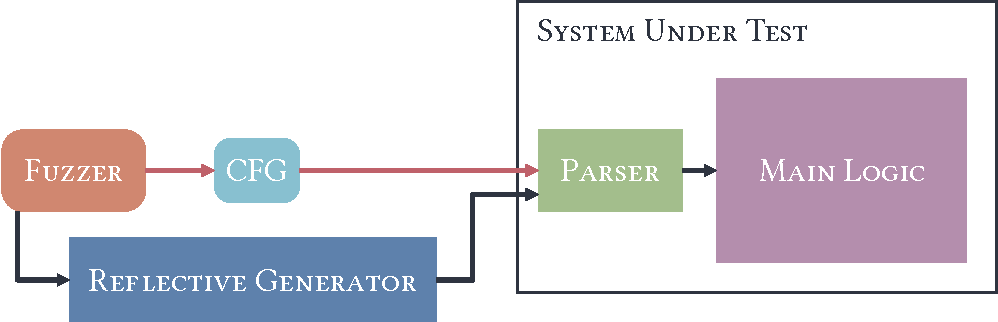
\includegraphics[width=.4\textwidth]{assets/fuzzing.pdf}
  \caption{Overview of gradually constrained fuzzing.}\label{fig:fuzzing-plan}
\end{wrapfigure}

Our system will start with a setup similar to Crowbar, but with a much greater
focus on the generators; in particular, we will use reflective generators to
gain significant testing power. The setup is shown in
Figure~\sectionref{fig:fuzzing-plan}. We start with a classic fuzzing setup, attempting
to make the system under test crash by passing it a variety of semi-random
inputs. Normally, the fuzzer is working against the parser, in the sense that
the parser's job is to reject invalid inputs and the fuzzer's job is to ``get
past the parser.'' The CFGs used by grammar-based fuzzers help a bit, but they
cannot generate inputs satisfying complex context-sensitive constraints. As in
Crowbar, we avoid this adversarial relationship and subsume grammar-based
generation with a powerful generator that is powerful enough to satisfy the
parser by construction; in our case, that generator is reflective.

Why use a reflective generator? First, we should clarify why any kind of monadic
generator is preferable to grammar-based options. Monadic generators can
straightforwardly generate context-free structures, and they can often do so
automatically with the help of type information~\cite{mista2019deriving}. If
this is all that the precondition requires, then there is no harm in using a
monadic generator, rather than a grammar-based one. But the beauty of a monadic
generator is that it can be made far more powerful, incrementally, as the
developer's testing needs change. The developer can start off thinking that they
need only consider the structure of their inputs, but they can later add more
semantic guarantees if they determine that their testing is ineffective.

Focusing on reflective generators specifically, one compelling benefit is that
their backward interpretation can be used to help seed the fuzzer.  Most fuzzers
ask for a number of {\em seeds}, input examples that the fuzzer can start from,
in order to ensure that the fuzzer does not spend ages exploring
inputs that have no hope of working out. Normally these seeds are easy enough
for the user to write down, since they are simply program inputs, but now that
we are asking the fuzzer to generate sequences of choices it becomes much more
error-prone (and tedious) to produce seeds by hand.  This is one great use for a
backward interpretation. The user can write down their seeds---either as values
in the program, or as text that can be parsed by the program's parser---and then
the reflective generator can reflect on the choices that produce those seeds.

The reflective generator also provides validity-preserving mutation. Guided by
heuristics, the system can opt to supplement the fuzzer's mutation schedule with
mutations that are obtained by the reflective generator's validity-preserving
mutation (which is more targeted than the mutators provided by the fuzzer). We
expect this to have a significant impact on performance, especially in contexts
where preconditions are relatively sparse and therefore hard for AFL++ to mutate
correctly.

Our ultimate goal is a grand unification of PBT and fuzzing generator tooling:
the fuzzing literature provides battle-tested heuristics for coverage-guided
generation, the PBT literature provides powerful tools like reflective
generators for refining generator performance incrementally, and both
communities benefit from generators with better distributions.

\SUBSECTION{Proposed Work: Reflective Shrinking}
A more modest application of reflective generators uses them to implement
validity-preserving {\em shrinking} of values to find smaller counterexamples
and speed up debugging. On its face, this feels similar to validity-preserving
mutation: Can we reflect on choices, shrink the choices, and then re-run the
generator with the smaller choices? Likely yes! But there are complications.
When mutating, it is often fine if the mutated value is accidentally quite
different from the original value, since the mutator is trying many values and
any that catch a bug are equally good. But when shrinking, it is often very
important to get another input that is both smaller and, ideally, provokes the
{\em same bug}. These nice properties are likely within reach, but care will
need to be taken to ensure that shrinkers behave as expected.

\SUBSECTION{Ongoing Work: Empirically Evaluating PBT Tools}
\amh{It's awkward to have ongoing work after proposed work, though I moved this
subsection up here because we are considering integrating it into the section on
generators as per our discussion over Slack.}
\bcp{If we're going to include the benchmarking project at all (and I
  think we should), we should ignore the fact that we've been working
  on it for a bit (after all, nothing is published or ready to
  publish) and talk aout it as proposed work.  At the same time, we
  should paint a big-picture vision for it, going somewhat beyond the
  ICFP submission we hope to make and talking about a real benchmark
  suite that we and others might build later.}

The many papers in the PBT literature demonstrate effectiveness with case
studies, showing that certain bugs in certain systems are caught more quickly
with one too over another. For theoretical advances, this is often sufficient
to demonstrate that the paper is worth publishing, but this kind of evaluation
can be hard to interpret from the perspective of a would-be user. \todo{Sentence
bridging to Jessica's paragraphs, linking in a theme from the intro}

\hg{Jessica is going to write us a couple of paragraphs for this}

\SECTION{Validation: Understanding Testing Effectiveness \pagebudget{3}}\label{sec:val}

One of the unique challenges in creating usable property-based testing is
providing adequate support for evaluating test results. Testing with properties
is fundamentally different from conventional unit testing tools in many ways.
First, it becomes a task in and of itself to understand individual inputs. This
because the inputs are not written by the developer, but rather generated
automatically, and furthermore, they can be of unbounded structural complexity.
Second, a developer needs to assess the quality of their tests. The quality of a
property-based test depends in part on the extent to which it covers execution
pathways through the code, though it also depends on the quality of the inputs.
Namely, are the inputs complex enough, and distributed in such a way that they
are likely to trigger practically important bugs? Third, developers need to
decide what to do with failed test cases, and may need to spend time migrating
failed test cases into regression suites. Finally, developers need to make
difficult decisions around how much computation time to budget for exercising
the property-based tests.

Each of these points of departure from conventional testing methodology
introduces new challenges into the testing process. And they require new
approaches to tool design to help developers reason about complex distributions
of complex inputs. In this section, we describe a sequence of research projects
we will undertake to bring about usable developer tooling for property-based
testing. These projects will contribute new paradigms for tools that help
developers understand program failures involving complex inputs
(Section~\ref{}), assess whether their generators are generating sufficient,
appropriate inputs (Section~\ref{}) and whether those inputs sufficiently
exercise their code (Section~\ref{}), migrate failed property-based tests into
regression tests (Section~\ref{}), and decide on compute budgets for their
property-based tests (Section~\ref{}). These projects will be pursued using
human-computer interaction methodology, integrating these tools into
contemporary development environments for functional programming. The result of
this work will be a comprehensive, innovative set of design primitives for
helping developers get work done in the challenge setting of reasoning about
tests with an overabundance of input-output examples.

% \amh{I think I want to organize this section chronologically around the
% following sequence of tasks: (1) understanding (and debugging) a single input;
% (2) understanding distributions of inputs; (3) tuning distributions of inputs;
% (4) integration of specific inputs into regression tests; (5) supporting good
% decisions around ``time budgets'' for PBT.}

\amh{Some notes on framing from a prior meeting with HG and BCP: When we write
about HCI-related parts of the projects, I think the right tack is to describe
this as an area of HCI-oriented programming tools that merits additional
exploration in tooling of the following types: X, Y, Z.  We will draw
inspiration from adjacent areas, though the idea is to establish some of the
first work in usable multi-example software testing.  This requires entirely new
ways of expressing and reviewing tests, and could have
potentially transformative impact within interactive programming systems in the
long term. (Can we flesh out just how big a field we feel this is?)}

\SUBSECTION{Proposed Work: Understanding Failures}

Once a PBT tool generates a counterexample of where a property fails, a
programmer will need to understand what in an input caused the program to fail.
This task can be rather challenging because generated inputs can be complex,
deep data structures \todo{Do we have a reference that implies the complexity of
generated counterexamples?}. Methods for making it clearer why a counterexample
fails could be to generate additional inputs that are very close to the
counterexample that are actually correct, to run the program up to the point
where the traces of the programs begin to diverge, and then to drop a programmer
into a debugging environment where they can query the state of the program and
step through the remainder of the execution. PI Head has prior work designing
debugging tools that help programmers understand trace divergences in an
educational setting~\cite{suzuki2017tracediff}.  \bcp{This sounds very cool!  We
should acknowledge all the work that's been done on shrinking in the PBT
community.} \amh{Good thinking!}
\hg{Hila had a similar idea that she wanted one of her undergrads to work on, we
should make sure we don't step on toes}\bcp{IMO the danger of stepping
on toes at this point is minimal---the time to worry about (and check) whose toes are
out there is when we actually start doing the work.}

\SUBSECTION{Proposed Work: Evaluating Input Distributions}
\newcommand{\genvis}{GenVis}

\amh{It might make sense for us to split out functionality
for tuning generator data distributions into a separate
section. I think the solutions to tuning data distributions
will require dedicated effort independent of the work to
develop useful visualizations of the distributions.}

\amh{In general, I think this proposal could be strengthened by: (1) emphasizing
needs that need to be satisfied with the tool (perhaps organizing the structure
of this subsubsection around those needs); and (2) proposing the features as
aspirational, rather than fixed, admitting in places where we don't know yet
what the right solution will be (for instance, I think it will take some work to
get a really good set of visualizations.)}
The work in \sectionref{sec:gen} will significantly improve the tools that
users have at their disposal when designing and using random generators, but
reflective generators do not solve all of the problems developers may run into
when writing generators. One common challenge is understanding when a random
generator successfully produces an interesting distribution of values. Many
participants in our study complained that they did not really know what their
generators were doing and asked for better tools for understanding the space of
inputs that the generator covers. Tools like this would help developers catch
mistakes that hamper their testing efforts and make it easier to quickly adapt
and tune their generators to their specific needs.

Of course, understanding generator distributions is challenging.  The values
produced by generators are often highly structured and have complex shapes
(think lists, trees, and other algebraic data types) \amh{I think the best
example of this I heard of during the interview study were lists of log events,
where each of those log events had multiple data fields---this would be really
hard to visualize without a bespoke visualization}.  Such values cannot simply
be plotted on a chart, and even spot-checking them visually may be hard if the
values are large.  Furthermore, writing generators is already considered by
developers to be a burden, so any tool in this space needs to be incredibly
automatic and easy to use.

\begin{wrapfigure}{r}{0.6\textwidth}
  \centering
  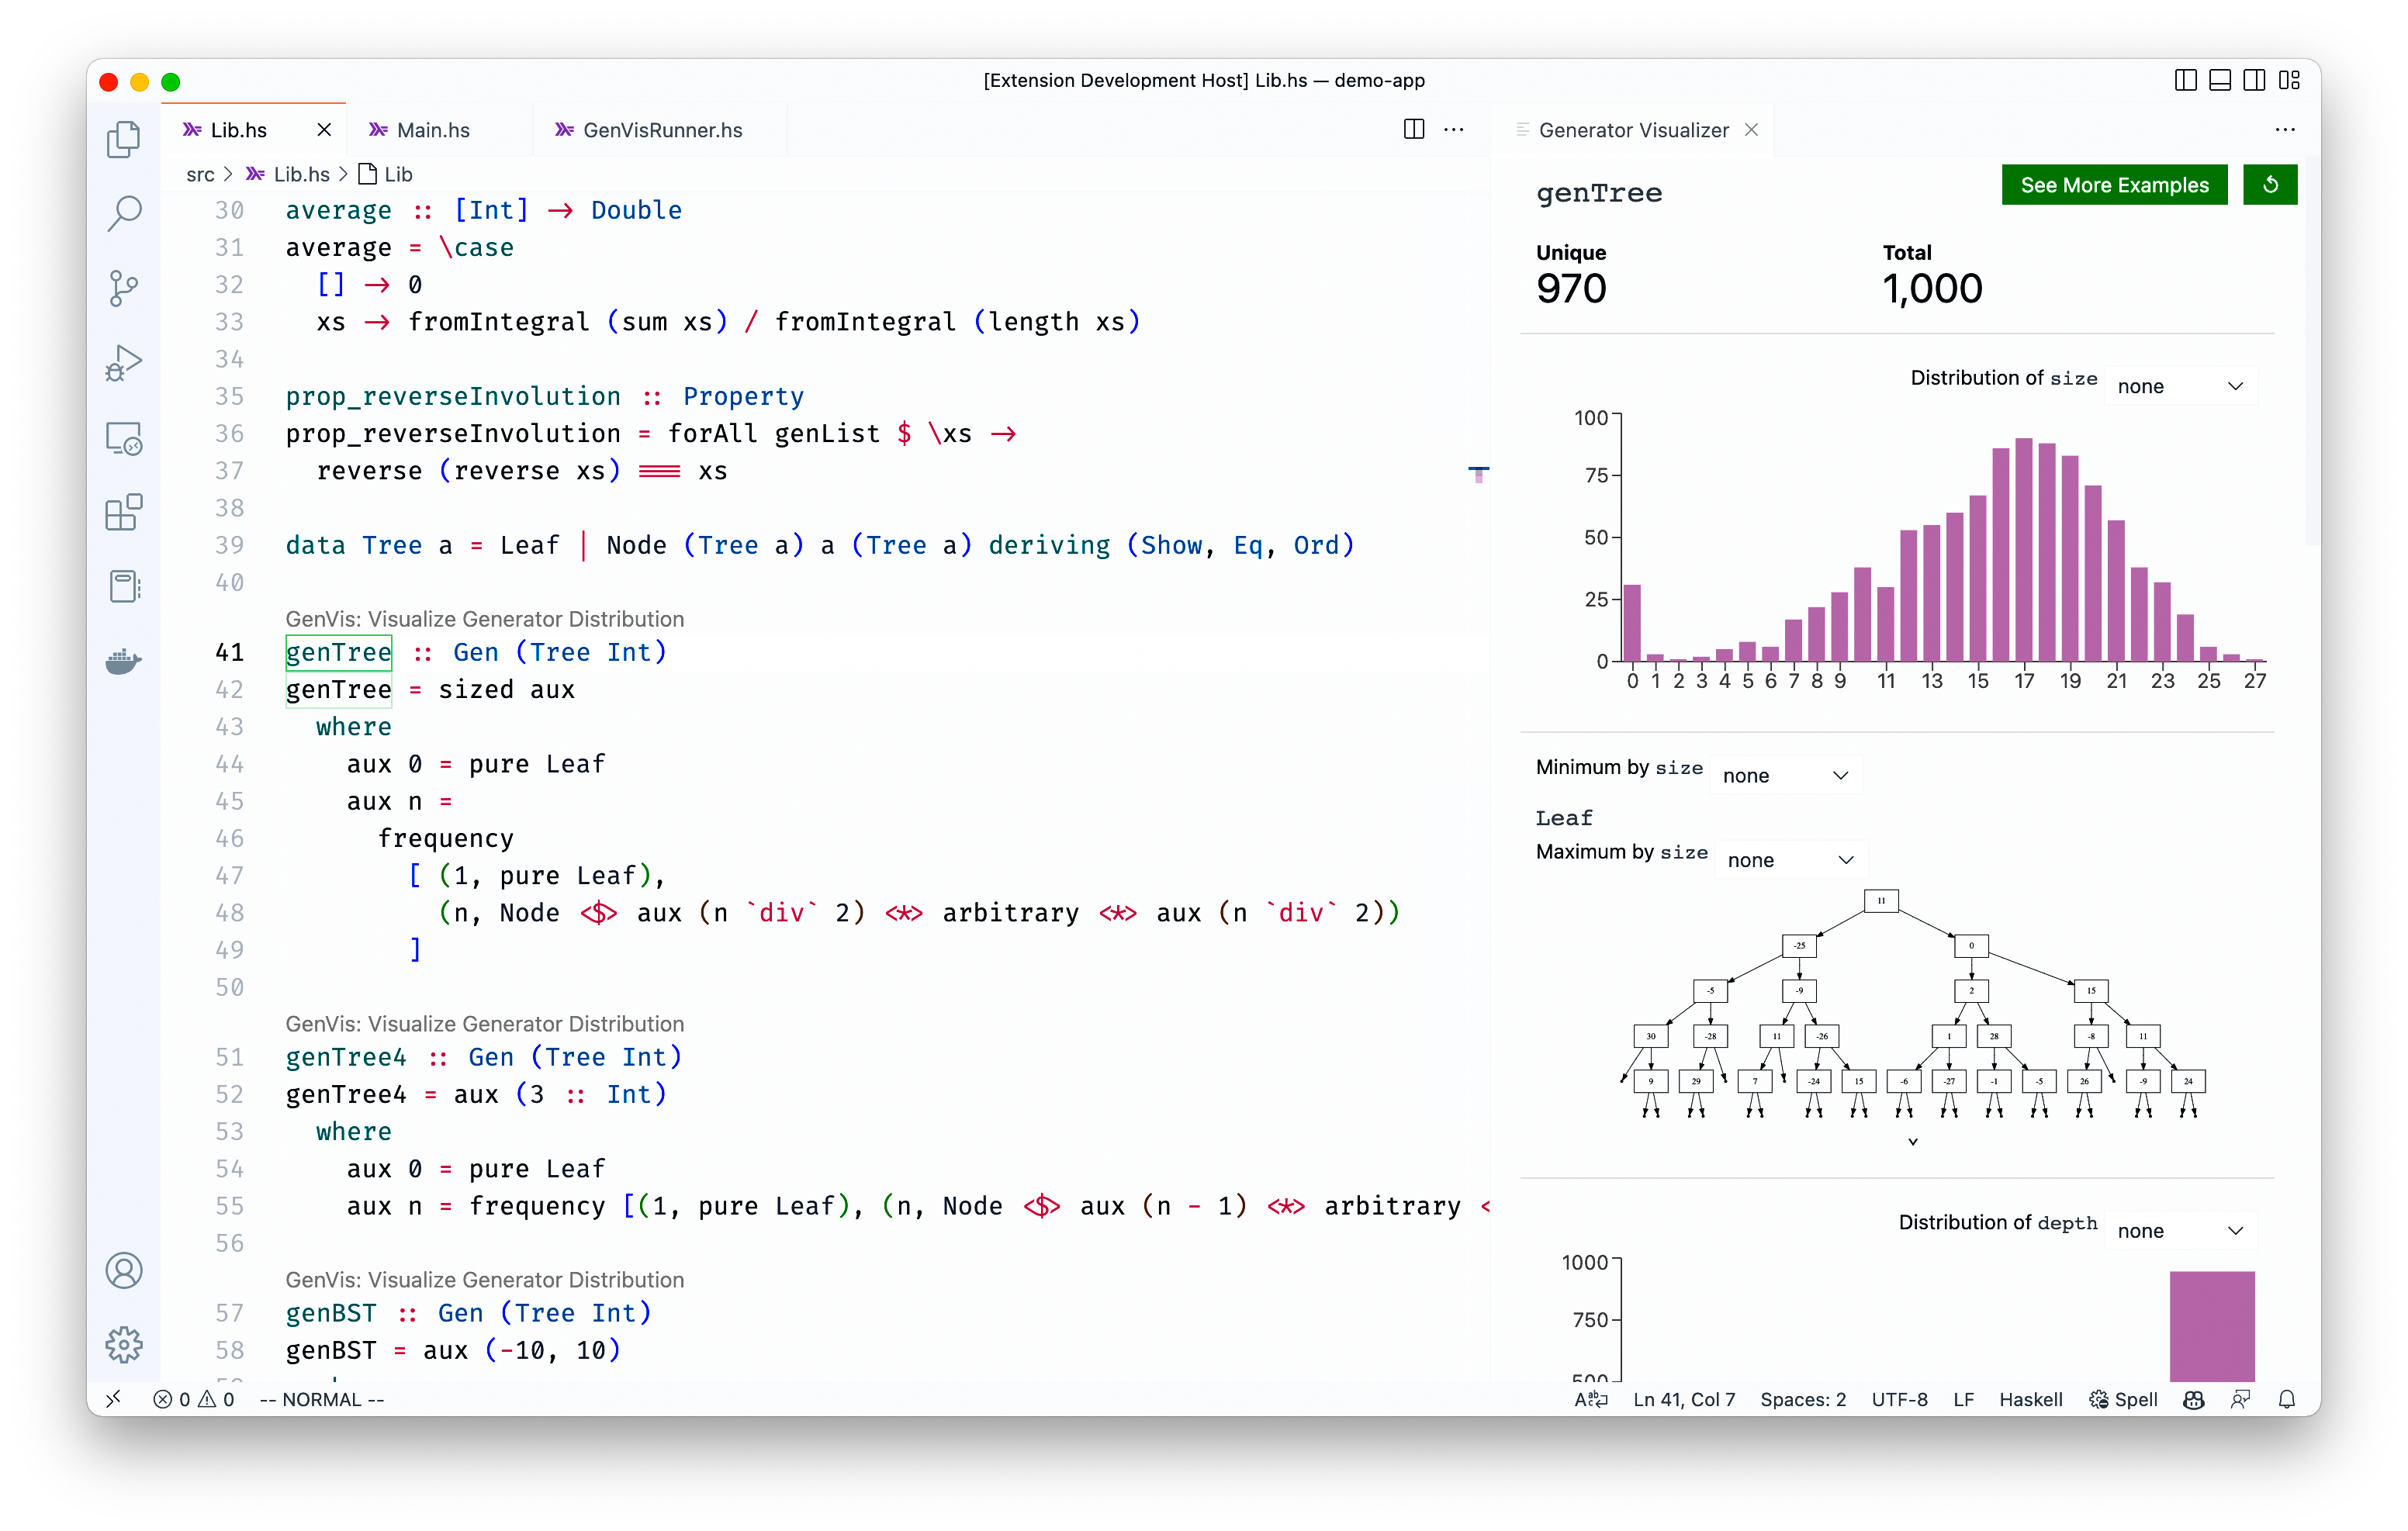
\includegraphics[width=0.6\textwidth]{assets/gen-vis.png}
  \caption{A mockup of \genvis.\amh{There is a lot
going on in this image, and I think it would help to zoom in a lot, and add
labels to the parts of the figure that represent key innovations, which you can
refer to from the text.} }\label{fig:gen-vis}
\end{wrapfigure}

With these challenges in mind, we propose to build \genvis, a tool that
gives developers comprehensive visualizations of their generators' distributions
from directly within their code editor. \genvis{} will address the challenges
with visualizing generator distributions by leveraging lightweight program
synthesis, visualization recommendation, and ideas from the live programming
literature.

\genvis{} starts by sampling a developer's generator and obtaining a set of
values to visualize. To get around the problem of arbitrarily structured data,
the system extracts and plots relevant {\em features} of a given datatype (e.g.,
for lists: length; for trees: size, depth, balance factor, etc.). \genvis{} will
start with a base set of features, extracted from the surrounding programming
environment and validated by the user; this will likely result in a few useful
visualizations, but maybe not enough. To ensure a comprehensive understanding of
the data, \genvis{} will then use lightweight program synthesis to compose and
combine the base of features to get {\em derived} features. The derived features
may features may show the relationship between different base features or even
compose base feature extractors to get entirely new features. \amh{Do you have
an example of a useful derived feature? I'm having a difficult time envisioning
a derived feature one would want to see, so it's less clear to me that this
feature will be useful.} All of the
features, base and derived, will be made available to users in a variety of
charts and graphs.

Of course, developers would struggle to grok dozens of charts representing
their data's features, so \genvis{} will also have a way for users to specify
which visualizations are interesting (and which to hide). We will base these
interactions based on the literature around visualization recommendation,
specifically Voyager~\cite{wongsuphasawat_voyager_2016,
wongsuphasawat_voyager_2017}. This interaction might be very quick (maybe a few
seconds to find a single representative chart) or slow and careful (many minutes
spent curating a dashboard of results to help with tuning), depending on how
much time and energy the developer has to put into their generator. Besides
charts, \genvis{} will also present the user with structured representations of
some generated values. We plan to use meta-programming to build
DOT graphs~\cite{ellson_graphviz_2002} that represent data types, and then
present those graphs to the developer for easier spot-checking of data.
\amh{The visualization skeptic in me wonders if it will be possible come up with
generalizable DOT-based visualizations that work out of the box for most data
types. I would expect most visualizations to become unreadable once the number
of nodes in the data structures surpasses 10. We need to make a stronger case
that our automated features (including proposed visualizations types of filters)
will regularly work on the kinds of complexity of the data people will generate,
or otherwise shift to a goal of supporting developers in rapid definition of
their own filters and visualizations.}

All of these features will be made available to developers from within their
editor as a VSCode extension, and they will update live as the programmer edits
their generator and adds new functions that are candidates for extracting base
features. We will evaluate \genvis{} in a small user study (~15 participants),
hoping to learn which features of the tool are most useful, and how the design
may be refined into a tool that real developers can use. \amh{What is our
strategy for getting this tool into the hands of real developers?}

\amh{Somewhere in this section we should emphasize the importance of helping
developers not just understand distributions in the aggregate, but also helping
them review individual examples, given that you need to see specific examples to
know that a generator is creating the right kind of data.}

\SUBSECTION{Proposed Work: Tuning Input Data Distributions}

\SUBSECTION{Proposed Work: Assessing Testing Effectiveness}

This section will include something about how to help
developers reason about whether their tests achieve adequate
code coverage. \amh{Discuss with Harry whether there is any
new approach we can achieve for code coverage, beyond
providing the kinds of metrics that appear from unit tests.
Maybe there are ways of automatically tuning input data
distributions so that they are more likely to execute path
through the code that a developer has indicated are
particularly important to exercise?}

\SUBSECTION{Proposed Work: Transforming Counterexamples into
Regression Tests}

\amh{Refer to Hila's work.} \amh{Discuss with Harry to
figure out if we have something novel to contribute here.
Perhaps it would involve novel technologies around
shrinkers.}

\SUBSECTION{Proposed Work: Running More Tests with Less Work}
% \SUBSECTION{Proposed Work: Integration with Continuous Integration Workflows}

The pilot study suggests that one area that new developer tooling may be
needed is in managing the interplay between PBT and continuous integration (CI)
systems. Recall that developers we spoke with pointed out frustration with the
fact that PBT is both nondeterministic and long-running. This combination left
them unsure of exactly where and when to test their properties: testing
properties locally slowed down their workflow, but testing them in CI
occasionally led them to find bugs at inconvenient times.

It is likely that PBT tools could play a role in improving this state of
affairs. For example, one could take inspiration from some theorem
provers~\cite{berghofer2004random} and create a system in which properties are
checked locally but in the background, as the programmer works on other things.
This avoids waiting time while potentially being less frustrating than running
in CI, since bugs would likely be found while the programmer still had the code
``paged in.'' Alternatively, one might design a PBT system with CI in mind,
providing automated features for deferring property failure notifications until
a specified time or turning failing properties into unit tests that can be saved
for future testing.

If the full-scale study indicates that this would be a useful line of work, we
will refine these ideas via user-centered design. Rather than build a system and
hope users like it, we will build minimal prototypes and iterate on the design
by observing testers using it. Ultimately we hope this will guide us to a tool
that will meaningfully improve the experience of PBT.

\SECTION{Education: Advancing Testing in the Broader Culture \pagebudget{1}}\label{sec:ed}

\hg{This isn't actually written, this is just starter stuff from my thesis
proposal}
The pilot study also reminded us that PBT builds on concepts that are not
always comfortable for developers, and we expect that we will learn more about
the specifics of that discomfort in the large-scale study.  Prior work has
explored ways to close this knowledge
gap~\cite{wrenn2021using,nelson2021automated}, but we expect there are further
education challenges that are worth exploring.

I hope to work with the course staff of CIS 1210 to incorporate PBT into the
curriculum. The ideal scenario would be to add a PBT thread throughout the
course, giving students the tools to specify and test their code as they go.  I
plan to follow the lead of others who have done similar things before (e.g., the
PL folks at Brown University) to give students the best chance at incorporating
PBT into their tool-set.

There are a few important challenges that need to be considered in order for
this to work out.  The curriculum is already quite full, so adding PBT likely
means removing something else. I will need to work with the professors currently
teaching the course to find room, but I expect that this process will be fairly
difficult. It is also possible that adding PBT will actually make parts of the
course {\em easier}, especially for students with some knowledge of logic and/or
less well-developed unit testing instincts. Honestly I think this is a good
thing, as it gives students more ways to succeed and it may re-enforce the value
of PBT, but some may find this problematic.

\SECTION{Plan of Work \pagebudget{.7}}\label{sec:plan-of-work}

\todo{(with a pretty pert chart or suchlike...)}

\SECTION{Broader Impacts \pagebudget{.5}}\label{sec:broader-impacts}
The Project Description must contain, as a separate section within the narrative, a section labeled ``Broader
Impacts of the Proposed Work". This section should provide a discussion of the broader impacts of the proposed
activities. Broader impacts may be accomplished through the research itself, through the activities that are
directly related to specific research projects, or through activities that are supported by, but are complementary to
the project. NSF values the advancement of scientific knowledge and activities that contribute to the
achievement of societally relevant outcomes. Such outcomes include, but are not limited to: full
participation of women, persons with disabilities, and underrepresented minorities in science, technology, engineering, and
mathematics (STEM); improved STEM education and educator development at any level; increased public
scientific literacy and public engagement with science and technology; improved well-being of individuals in
society; development of a diverse,globally competitive STEM workforce; increased partnerships between
academia, industry, and others; improved national security; increased economic competitiveness of the United
States; and enhanced infrastructure for research and education.

\SECTION{Results from Prior NSF Support \pagebudget{.5}}
If any PI or co-PI identified on the project has received NSF funding (including any current
funding) in the past five years, in formation on the award(s) is required,
irrespective of whether the support was directly related to the proposal or not.
In cases where the PI or co-PI has received more than one award (excluding amendments),
they need only report on the one award most closely related to the proposal. Funding includes not just salary
support, but any funding awarded by NSF. The following information must be provided:\\

\noindent
\emph{\underline{Name of PI}}: NSF-Program (Award Number) ``Title of the Project'' (\$AMOUNT, PERIOD OF SUPPORT).
{\bf Publications:} List of publications resulting from the NSF award. A complete bibliographic citation for each
publication must be provided either in this section or in the References Cited section of the proposal); if
none, state: ``No publications were produced under this award.'' {\bf Research Products:} evidence of research products
and their availability, including, but not limited to: data, publications, samples, physical collections, software,
and models, as described in any Data Management Plan.

% \SUBSECTION{Proposed Study}
% The Project Description should provide a clear statement of the work to be undertaken and must include:
% objectives for the period of the proposed work and expected significance; relation to longer-term goals of the PI's
% project; and relation to the present state of knowledge in the field, to work in progress by the PI under other
% support and to work in progress elsewhere.
%
% The Project Description should outline the general plan of work, including the broad design of activities to be
% undertaken, and, where appropriate, provide a clear description of experimental methods and procedures.
% Proposers should address what they want to do, why they want to do it, how they plan to do it, how they will
% know if they succeed, and what benefits could accrue if the project is successful. The project activities may be
% based on previously established and/or innovative methods and approaches, but in either case must be well
% justified. These issues apply to both the technical aspects of the proposal and the way in which the project may
% make broader contributions.

\iflater
\section*{More stuff to not forget :-)}

Unfunded collaborations: Any substantial collaboration with
individuals not included in the budget should be described in the
Facilities, Equipment and Other Resources section of the proposal (see
Chapter II.C.2.i) and documented in a letter of collaboration from
each collaborator. Such letters should be provided in the
supplementary documentation section of FastLane or Research.gov and
follow the format instructions specified in Chapter
II.C.2.j. Collaborative activities that are identified in the budget
should follow the instructions in Chapter II.D.3.  \bcp{Jane Street.
  And maybe we should ask John too?}

bpc.net - source materials for NSF BPC plans (they also vet plans).
  we should check that other universities are doing!

\fi
